%  LaTeX support: latex@mdpi.com 
%  In case you need support, please attach all files 
%  that are necessary for compiling as well as the log file, 
%  and specify the details of your LaTeX setup 
%  (which operating system and LaTeX version / tools you are using).

%=================================================================
\documentclass[ijgi,article,submit,moreauthors,pdftex]{Definitions/mdpi} 


%=================================================================
\firstpage{1} 
\makeatletter 
\setcounter{page}{\@firstpage} 
\makeatother
\pubvolume{xx}
\issuenum{1}
\articlenumber{5}
\pubyear{2019}
\copyrightyear{2019}
%\externaleditor{Academic Editor: name}
\history{Received: date; Accepted: date; Published: date}
%\updates{yes} % If there is an update available, un-comment this line

%% MDPI internal command: uncomment if new journal that already uses continuous page numbers 
%\continuouspages{yes}

%------------------------------------------------------------------
% The following line should be uncommented if the LaTeX file is uploaded to arXiv.org
%\pdfoutput=1

%=================================================================
% Add packages and commands here. The following packages are loaded in our class file: fontenc, calc, indentfirst, fancyhdr, graphicx, lastpage, ifthen, lineno, float, amsmath, setspace, enumitem, mathpazo, booktabs, titlesec, etoolbox, amsthm, hyphenat, natbib, hyperref, footmisc, geometry, caption, url, mdframed, tabto, soul, multirow, microtype, tikz

\usepackage{xspace}
\usepackage{mathtools}
\usepackage{fancyvrb} %for \begin{Verbatim} environment; color in verbatime



\usepackage{xcolor,listings}
\usepackage{textcomp}
\lstset{upquote=true}






%\usepackage[T1]{fontenc}
%\usepackage{subcaption}
%=================================================================
%% Please use the following mathematics environments: Theorem, Lemma, Corollary, Proposition, Characterization, Property, Problem, Example, ExamplesandDefinitions, Hypothesis, Remark, Definition, Notation, Assumption
%% For proofs, please use the proof environment (the amsthm package is loaded by the MDPI class).

%so that we have more tolerance for large figures
%large figure is less likely to push to the end of the document
\renewcommand{\textfraction}{0.01}
\renewcommand{\topfraction}{0.99}
\renewcommand{\bottomfraction}{0.99}
\renewcommand{\dbltopfraction}{0.99} % fit big float above 2-col. text

\graphicspath{{images/}}

\newcommand{\astar}{A$^{\!\star}$\xspace}

\newcommand{\e}[1]{\times 10^{#1}}
\newcommand{\fig}{Figure~}
\newcommand{\eq}{Equation~}
\newcommand{\fo}{Formula~}
\newcommand{\sect}{Section~}
\newcommand{\tbl}{Table~}
\newcommand{\chap}{Chapter~}
\newcommand{\figs}{Figures~}
\newcommand{\eqs}{Equations~}
\newcommand{\fos}{Formulas~}
\newcommand{\sects}{Sections~}
\newcommand{\tbls}{Tables~}
\newcommand{\chaps}{Chapters~}
\newcommand{\eg}{e.g.,~}
\newcommand{\ie}{i.e.,~}
\newcommand{\p}{p.~}
\newcommand{\pp}{pp.~}

\makeatletter
\def\verbatim@font{\normalfont\rmfamily}
\makeatother


%=================================================================
% Full title of the paper (Capitalized)
\Title{Paralleling Generalization Operations to Support Smooth Zooming:
Case Study of Merging Land-Cover Areas}
%\Title{Merging land-cover areas parallelly 
%to support smooth zooming of web maps}

% Author Orchid ID: enter ID or remove command
\newcommand{\orcidauthorA}{0000-0000-000-000X} % Add \orcidA{} behind the author's name
%\newcommand{\orcidauthorB}{0000-0000-000-000X} % Add \orcidB{} behind the author's name

% Authors, for the paper (add full first names)
\Author{
Firstname Lastname $^{1,\dagger,\ddagger}$\orcidA{}, 
Firstname Lastname $^{1,\ddagger}$ and 
Firstname Lastname $^{2,}$*}

% Authors, for metadata in PDF
\AuthorNames{Firstname Lastname, Firstname Lastname and Firstname Lastname}

% Affiliations / Addresses (Add [1] after \address if there is only one affiliation.)
\address{%
$^{1}$ \quad Affiliation 1; e-mail@e-mail.com\\
$^{2}$ \quad Affiliation 2; e-mail@e-mail.com}

% Contact information of the corresponding author
\corres{Correspondence: e-mail@e-mail.com; Tel.: (optional; include country code; 
if there are multiple corresponding authors, add author initials) +xx-xxxx-xxx-xxxx (F.L.)}

% Current address and/or shared authorship
\firstnote{Current address: Affiliation 3} 
\secondnote{These authors contributed equally to this work.}
% The commands \thirdnote{} till \eighthnote{} are available for further notes

%\simplesumm{} % Simple summary

%\conference{} % An extended version of a conference paper

% Abstract (Do not insert blank lines, i.e. \\) 
\abstract{
abstract
}

% Keywords
\keyword{many keywords}



%%%%%%%%%%%%%%%%%%%%%%%%%%%%%%%%%%%%%%%%%%
% Only for the journal Data:
%\dataset{DOI number or link to the deposited data set in cases where the data set is published or set to be published separately. If the data set is submitted and will be published as a supplement to this paper in the journal Data, this field will be filled by the editors of the journal. In this case, please make sure to submit the data set as a supplement when entering your manuscript into our manuscript editorial system.}

%\datasetlicense{license under which the data set is made available (CC0, CC-BY, CC-BY-SA, CC-BY-NC, etc.)}



%\setcounter{secnumdepth}{4}
%%%%%%%%%%%%%%%%%%%%%%%%%%%%%%%%%%%%%%%%%%
\begin{document}
%%%%%%%%%%%%%%%%%%%%%%%%%%%%%%%%%%%%%%%%%%



\section{Introduction}

my introduction

\cite{Mackaness2017Generalization}


 
\section{Related Work}
\label{sec:realted_work}

my Related Work


\section{Methodology}
\label{sec:methodology}


my methodology




\subsection{A Greedy Algorithm}
\label{sec:greedy_algo}


my algorithm



\section{Case Study}
\label{sec:case_study}


my case study





\section{Concluding Remarks}
\label{sec:concluding_remarks}

\subsection{Conclusion}



\subsection{Future Work}

my future work

\section{Evaluation}

\subsection{Type Change}

When we aggregate land-cover polygon~$p$ into land-cover polygon~$q$,
the type of~$p$ is changed to the type of~$q$.  
We define the cost of type change as
\begin{equation}
\label{eq:f_type}
f_\mathrm{type}(p,q)=a_p \cdot d_\mathrm{type}(T(p),T(q)),
\end{equation}
where $a_p$ is the area of land-cover polygon~$p$. 
Expressions~$T(p)$ and~$T(q)$ denote the types of the two polygons, respectively.
Formula~$d_\mathrm{type}(T(p),T(q))$ is the distance of the two types;
\fig\ref{fig:evaluations_type_distance} shows an example of type distances.

\begin{figure*}[tb]
\centering
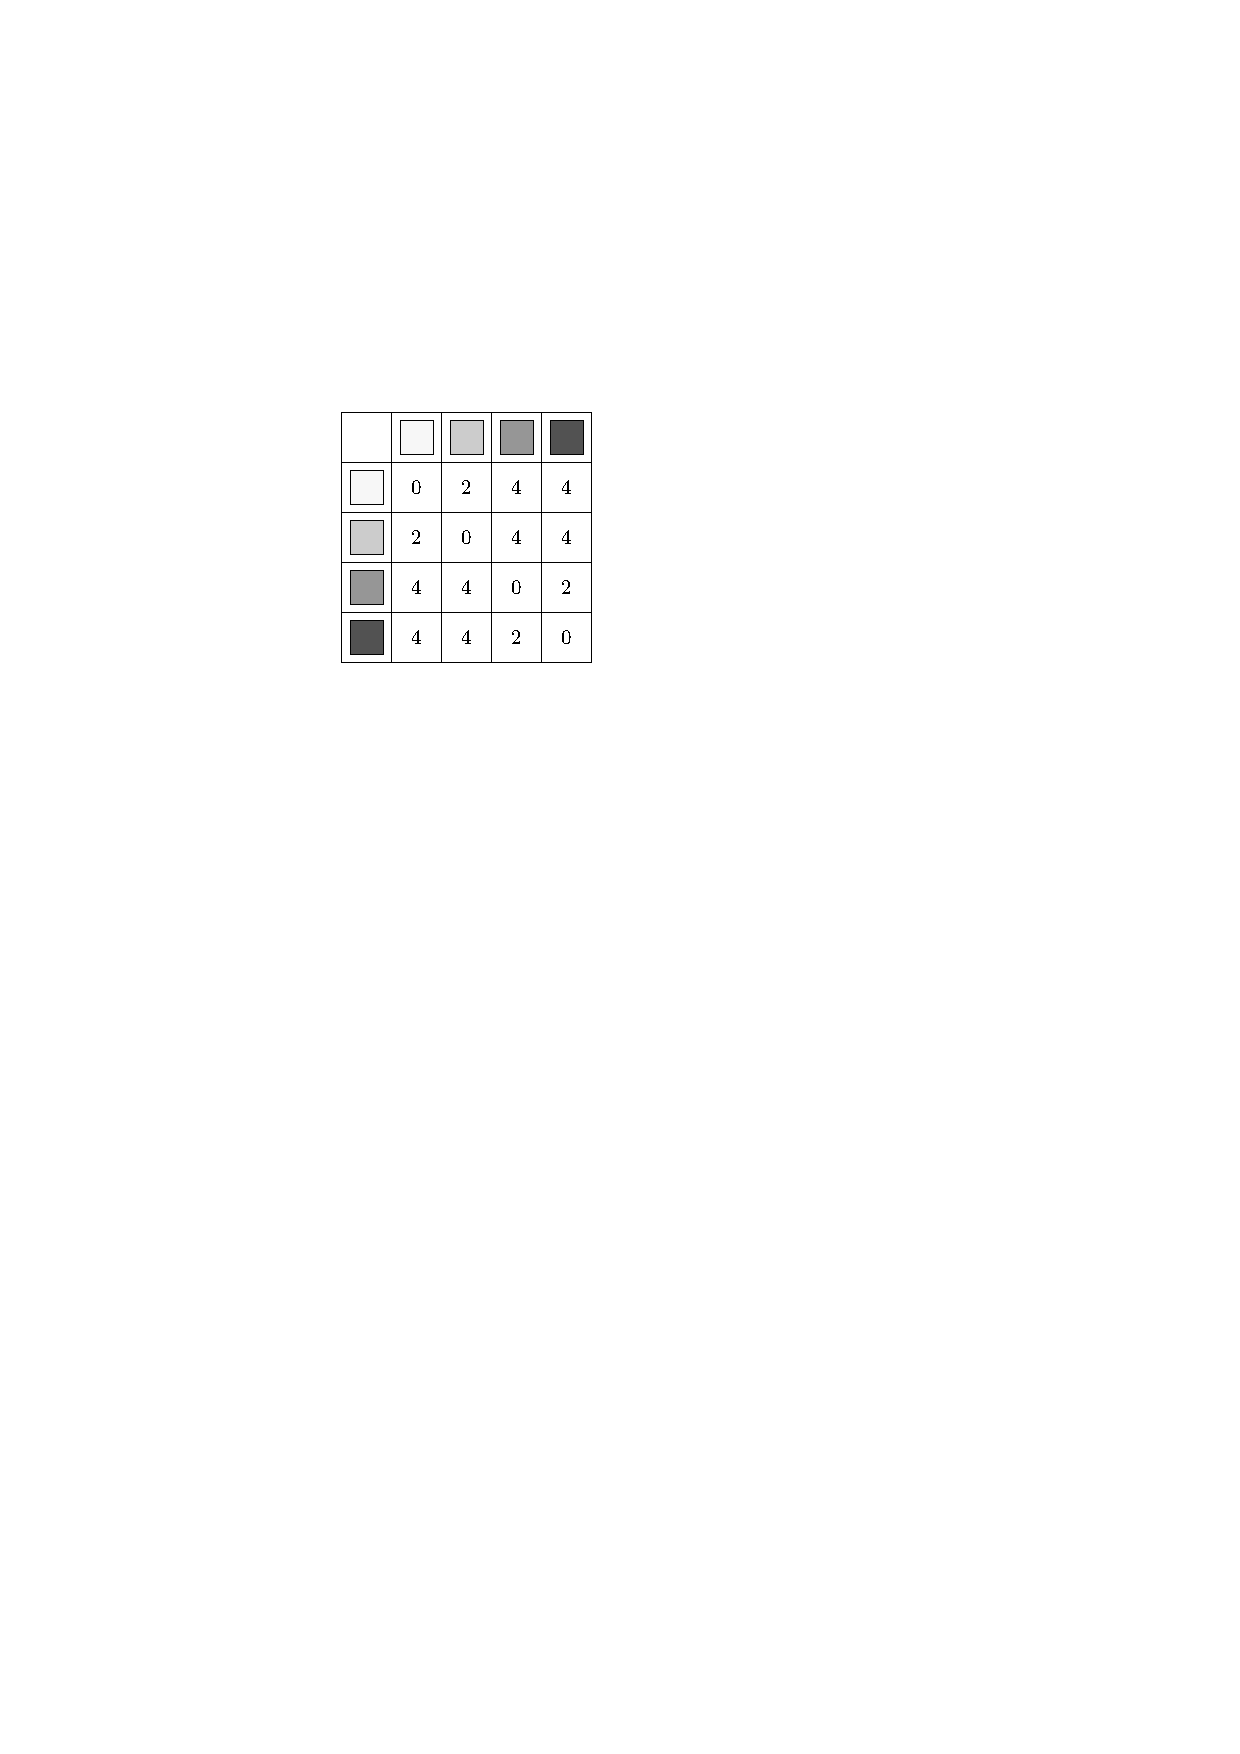
\includegraphics[page=1]{evaluations}
\caption{An example of type distances of land-cover polygons, 
    where each color represents a type.
}
\label{fig:evaluations_type_distance}
\end{figure*}


We have two preferences for the type change when we generate intermediate maps.
First, the changes of each step should be small.
Take \fig\ref{fig:evaluations} for example, the corresponding polygons of
set~$C_{2,1}$ (the relevant places after  changing) and 
set~$C_{1,2}$ (the relevant places before changing)
should be similar in terms of land-cover types.
Therefore, we define the cost of type change of a step,
from state~$s-1$ to state~$s$, as
\begin{equation}
\label{eq:F_type}
F_\mathrm{type}(s)=\sum_{i=1}^{|C_{s-1,s}|} f_\mathrm{type}(p_i,q_i),
\end{equation}
where corresponding polygons~$p_i$ and~$q_i$ are respectively from 
the two sets of changed polygons~$C_{s-1,s}$ and~$C_{s,s-1}$.
There holds~$|C_{s-1,s}| = |C_{s,s-1}|$.
According to the type distances defined in \fig\ref{fig:evaluations_type_distance},
we have~$F_\mathrm{type}(2)=120$
for type changes from set~$C_{1,2}$ to set~$C_{2,1}$ 
(see \fig\ref{fig:evaluations}), and
we have~$F_\mathrm{type}(3)=82$
for type changes, from set~$C_{2,3}$ to set~$C_{3,2}$.


Our second preference for the type change is that 
the differences between an intermediate map and the start map
should be small.
Take \fig\ref{fig:evaluations} for example, the corresponding polygons of
set~$C'_{3,1}$ (the relevant places after  changing) and 
set~$C'_{1,3}$ (the relevant places before changing)
should be similar in terms of land-cover types.
We define this cost, from state~$1$ to state~$s$, as
\begin{equation}
\label{eq:F_type_prime}
F'_\mathrm{type}(s)=\sum_{i=1}^{|C'_{1,s}|} f_\mathrm{type}(p'_i,q'_i),
\end{equation}
where corresponding polygons~$p'_i$ and~$q'_i$ are respectively from 
the two sets of changed polygons~$C'_{1,s}$ and~$C'_{s,1}$.
There holds~$|C'_{1,s}| = |C'_{s,1}|$.
According to the type distances defined in \fig\ref{fig:evaluations_type_distance},
we have~$F'_\mathrm{type}(3)=172$
for type changes, from set~$C'_{1,3}$ to set~$C'_{3,1}$
(see \fig\ref{fig:evaluations}).

\subsection{Length Change}

{\color{red}the length should not decrease evenly. 
Instead, it should decrease evenly on map.}

We also have two preferences for the shape when we generate intermediate maps.
First, the interior length should decrease evenly from the current map.
Take \fig\ref{fig:evaluations} for example, 
from state~$s=3$ the interior length should decrease by~$12$ at each step.
Therefore, we define the cost of length change of a step,
from state~$s-1$ to state~$s$, as
\begin{equation}
\label{eq:F_lgth}
F_\mathrm{lgth}(s)=
    \left(\ell_\mathrm{int}(s-1)-\ell_\mathrm{int}(s)-
        \frac{\ell_\mathrm{int}(s-1)}{n_\mathrm{state}-s+1}\right)^2,
\end{equation}
where expression~$\ell_\mathrm{int}(s-1)-\ell_\mathrm{int}(s)$ 
is the decrease of interior length from state~$s-1$ to state~$s$.
Parameter~$n_\mathrm{state}$ denotes the total number of states.
Expression~$\frac{\ell_\mathrm{int}(s-1)}{n_\mathrm{state}-s+1}$
is the average decrease of interior length from state~$s-1$ 
to a map with all the polygons merged.
Take \fig\ref{fig:evaluations} for example,
we have~$n_\mathrm{state}=5$ and~$F_\mathrm{lgth}(3)=\frac{16}{9}$.


Our second preference of for the shape is that
the interior length should decrease evenly from the start map. 
Take \fig\ref{fig:evaluations} for example, 
from time~$state=1$ the interior length should decrease by~$11$ at each step.
We define this cost as
\begin{equation}
\label{eq:F_lgth_prime}
F'_\mathrm{lgth}(s)=
\left(\ell_\mathrm{int}(s-1)-\ell_\mathrm{int}(s)-
        \frac{\ell_\mathrm{int}(1)}{n_\mathrm{state}-1}\right)^2,
\end{equation}
where expression~$\frac{\ell_\mathrm{int}(1)}{n_\mathrm{step}-1}$
is the average decrease of interior length from state~$s=1$ 
to a map with all the polygons merged.
Take \fig\ref{fig:evaluations} for example,
we have~$F'_\mathrm{lgth}(3)=1$.

We define the total cost of the whole aggregation sequence
based on \eqs\ref{eq:F_type}, \ref{eq:F_type_prime}, 
\ref{eq:F_lgth}, and \ref{eq:F_lgth_prime}. 
That is,
\begin{equation}
\label{eq:F}
F = \sum_{s=2}^{n_\mathrm{state}}
        \bigg(
            (2-\lambda)F_\mathrm{type}(s) +
            (2-\lambda)F'_\mathrm{type}(s) + 
            \lambda F_\mathrm{lgth}(s) +
            \lambda F'_\mathrm{lgth}(s)
        \bigg),
%F = \sum_{s=2}^{n_\mathrm{state}}
%        \left( 
%            (2-\lambda)F_\mathrm{type}(s) +
%            (2-\lambda)F'_\mathrm{type}(s) + 
%            \frac{\lambda d_\mathrm{type\_max}}{2} F_\mathrm{lgth}(s) +
%            \frac{\lambda d_\mathrm{type\_max}}{2}F'_\mathrm{lgth}(s)
%        \right),
\end{equation}
where parameter~$\lambda$ $(0\le \lambda \le 2)$ can be used to assign the importances of 
type change and length change.
In our experiment, we set $\lambda=1$.
%Constant~$d_\mathrm{type\_max}$ is the maximum distance between two land-cover types,
%which is known from input.
%For example,
%we have~$d_\mathrm{type\_max}=4$ for the instance of \fig\ref{fig:evaluations_type_distance}.
%We use expression~$\frac{d_\mathrm{type\_max}}{2}$ to, hopefully, 
%make the cost of type change and the cost of length change comparable.

We use the interior length instead of the compactness to define the cost of shape
because we think the interior length is more versatile.
By contrast, some land-cover polygons like shapes with high compactnesses 
(e.g., forests and lakes),
while some other land-cover polygons like shapes with low compactnesses 
(e.g., roads and rivers).


\begin{figure*}[tb]
\centering
\includegraphics[page=2]{evaluations}
\caption{Some examples to illustrate how to compute the costs of an aggregation sequence.
}
\label{fig:evaluations}
\end{figure*}



\section{Conclusion}
We considered only two operations: split and merge.
One may need to extend our method according to their demands.


%When we remove a triangle by slicing the SSC, 
%we may want to keep three vertices of the triangle 
%instead of making four vertices.
%In this case, the polyhedron (with five faces) should have curly edges,
%which is also known as a \emph{curved polyhedron}.
%The slopes of curly edges need to be studied.







































%Some research questions are as follows.
%What aspects should we optimize 
%(e.g., minimizing the number of merging events or 
%assigning similar numbers of merging steps to each event)?
%What algorithm should we use 
%(e.g., dynamic programming, \Astar, or integer linear programming)?
%How much time is gained for users to observe the merging steps on the screen?
%How to store the parallel merging steps?









%%%%%%%%%%%%%%%%%%%%%%%%%%%%%%%%%%%%%%%%%%%
%\section{Patents}
%This section is not mandatory, but may be added if there are patents resulting from the work reported in this manuscript.
%
%%%%%%%%%%%%%%%%%%%%%%%%%%%%%%%%%%%%%%%%%%%
%\vspace{6pt} 
%
%%%%%%%%%%%%%%%%%%%%%%%%%%%%%%%%%%%%%%%%%%%
%%% optional
%%\supplementary{The following are available online at \linksupplementary{s1}, Figure S1: title, Table S1: title, Video S1: title.}
%
%% Only for the journal Methods and Protocols:
%% If you wish to submit a video article, please do so with any other supplementary material.
%% \supplementary{The following are available at \linksupplementary{s1}, Figure S1: title, Table S1: title, Video S1: title. A supporting video article is available at doi: link.}
%
%%%%%%%%%%%%%%%%%%%%%%%%%%%%%%%%%%%%%%%%%%%
%\authorcontributions{For research articles with several authors, a short paragraph specifying their individual contributions must be provided. The following statements should be used ``conceptualization, X.X. and Y.Y.; methodology, X.X.; software, X.X.; validation, X.X., Y.Y. and Z.Z.; formal analysis, X.X.; investigation, X.X.; resources, X.X.; data curation, X.X.; writing--original draft preparation, X.X.; writing--review and editing, X.X.; visualization, X.X.; supervision, X.X.; project administration, X.X.; funding acquisition, Y.Y.'', please turn to the  \href{http://img.mdpi.org/data/contributor-role-instruction.pdf}{CRediT taxonomy} for the term explanation. Authorship must be limited to those who have contributed substantially to the work reported.}
%
%%%%%%%%%%%%%%%%%%%%%%%%%%%%%%%%%%%%%%%%%%%
%\funding{Please add: ``This research received no external funding'' or ``This research was funded by NAME OF FUNDER grant number XXX.'' and  and ``The APC was funded by XXX''. Check carefully that the details given are accurate and use the standard spelling of funding agency names at \url{https://search.crossref.org/funding}, any errors may affect your future funding.}
%
%%%%%%%%%%%%%%%%%%%%%%%%%%%%%%%%%%%%%%%%%%%
%\acknowledgments{In this section you can acknowledge any support given which is not covered by the author contribution or funding sections. This may include administrative and technical support, or donations in kind (e.g., materials used for experiments).}
%
%%%%%%%%%%%%%%%%%%%%%%%%%%%%%%%%%%%%%%%%%%%
%\conflictsofinterest{Declare conflicts of interest or state ``The authors declare no conflict of interest.'' Authors must identify and declare any personal circumstances or interest that may be perceived as inappropriately influencing the representation or interpretation of reported research results. Any role of the funders in the design of the study; in the collection, analyses or interpretation of data; in the writing of the manuscript, or in the decision to publish the results must be declared in this section. If there is no role, please state ``The funders had no role in the design of the study; in the collection, analyses, or interpretation of data; in the writing of the manuscript, or in the decision to publish the results''.} 
%
%%%%%%%%%%%%%%%%%%%%%%%%%%%%%%%%%%%%%%%%%%%
%%% optional
%\abbreviations{The following abbreviations are used in this manuscript:\\
%
%\noindent 
%\begin{tabular}{@{}ll}
%MDPI & Multidisciplinary Digital Publishing Institute\\
%DOAJ & Directory of open access journals\\
%TLA & Three letter acronym\\
%LD & linear dichroism
%\end{tabular}}
%
%%%%%%%%%%%%%%%%%%%%%%%%%%%%%%%%%%%%%%%%%%%
%%% optional
%\appendixtitles{no} %Leave argument "no" if all appendix headings stay EMPTY (then no dot is printed after "Appendix A"). If the appendix sections contain a heading then change the argument to "yes".
%\appendix
%\section{}
%\unskip
%\subsection{}
%The appendix is an optional section that can contain details and data supplemental to the main text. For example, explanations of experimental details that would disrupt the flow of the main text, but nonetheless remain crucial to understanding and reproducing the research shown; figures of replicates for experiments of which representative data is shown in the main text can be added here if brief, or as Supplementary data. Mathematical proofs of results not central to the paper can be added as an appendix.
%
%\section{}
%All appendix sections must be cited in the main text. In the appendixes, Figures, Tables, etc. should be labeled starting with `A', e.g., Figure A1, Figure A2, etc. 

%%%%%%%%%%%%%%%%%%%%%%%%%%%%%%%%%%%%%%%%%%
% Citations and References in Supplementary files are permitted provided that they also appear in the reference list here. 

%=====================================
% References, variant A: internal bibliography
%=====================================
%\reftitle{References}
%\begin{thebibliography}{999}
%% Reference 1
%\bibitem[Author1(year)]{ref-journal}
%Author1, T. The title of the cited article. {\em Journal Abbreviation} {\bf 2008}, {\em 10}, 142--149.
%% Reference 2
%\bibitem[Author2(year)]{ref-book}
%Author2, L. The title of the cited contribution. In {\em The Book Title}; Editor1, F., Editor2, A., Eds.; Publishing House: City, Country, 2007; pp. 32--58.
%\end{thebibliography}
\bibliography{Reference/BibReference}

% The following MDPI journals use author-date citation: Arts, Econometrics, Economies, Genealogy, Humanities, IJFS, JRFM, Laws, Religions, Risks, Social Sciences. For those journals, please follow the formatting guidelines on http://www.mdpi.com/authors/references
% To cite two works by the same author: \citeauthor{ref-journal-1a} (\citeyear{ref-journal-1a}, \citeyear{ref-journal-1b}). This produces: Whittaker (1967, 1975)
% To cite two works by the same author with specific pages: \citeauthor{ref-journal-3a} (\citeyear{ref-journal-3a}, p. 328; \citeyear{ref-journal-3b}, p.475). This produces: Wong (1999, p. 328; 2000, p. 475)

%=====================================
% References, variant B: external bibliography
%=====================================
%\externalbibliography{yes}
%\bibliography{your_external_BibTeX_file}

%%%%%%%%%%%%%%%%%%%%%%%%%%%%%%%%%%%%%%%%%%
%% optional
%\sampleavailability{Samples of the compounds ...... are available from the authors.}

%% for journal Sci
%\reviewreports{\\
%Reviewer 1 comments and authors’ response\\
%Reviewer 2 comments and authors’ response\\
%Reviewer 3 comments and authors’ response
%}




%%%%%%%%%%%%%%%%%%%%%%%%%%%%%%%%%%%%%%%%%%
\end{document}

